\iffalse\documentclass{article}\fi
\documentclass[12pt]{article}

\usepackage{sbc-template}
\usepackage{graphicx,url}

%sudo apt install texlive-lang-portuguese
\usepackage[brazilian]{babel}   
\usepackage[utf8]{inputenc} 

\usepackage{graphicx}

%\usepackage[numbib,nottoc]{blindtext}
%\usepackage[numbib,nottoc]{tocbibind}

\graphicspath{ {./images/} }

\sloppy

\title{Avaliação de superpixels para segementação de imagens}

%Avaliar se superpixels podem ser utilizadas na segmentação de imagens sem diminuição do desempenho da segmentação, porém com custo inferior.

\author{Felipe Augusto Lima Reis\inst{1}}

\address{PUC Minas - Pontifícia Universidade Católica de Minas Gerais
  \email{falreis@sga.pucminas.br} }

\begin{document} 

\maketitle

\begin{abstract}
  Superpixels are structures that group similar pixels into sets that reflect aspects of the image. This article evaluates the use of SLICO superpixels and partition hierarchy for segmentation. Using \textbf{neural networks} for segmentation, the results of superpixels images with different levels of granularity and untreated images were compared to the ground-truth. The article also evaluates the training time of neural networks for superpixels based images. For training and evaluation, the Berkeley Segmentation Data Set (BSDS500) \cite{BSDS500} image was used.
\end{abstract}
     
\begin{resumo} 
  Superpixels são estruturas que agrupam pixels semelhantes em conjuntos que refletem aspectos da imagem. Este artigo avalia a utilização superpixels SLICO e hierarquia de partições para segmentação. Utilizando \textbf{redes neurais} para segmentação, os resultados de imagens utilizando superpixels com diferentes níveis de granularidade e imagens sem tratamento foram comparadas em relação ao \textit{ground-truth}. O artigo também avalia o tempo de treinamento das redes neurais para imagens com superpixels em relação às imagens originais. Para treinamento e avaliação foram utilizadas imagem do Berkeley Segmentation Data Set (BSDS500) \cite{BSDS500}.
\end{resumo}


\section{Introdução} \label{sec:introducao}

O presente trabalho apresenta a seguinte estrutura: a Seção \ref{sec:ref_teorico} mostra o referencial teórico para construção do trabalho, a Seção  \ref{sec:mat_metodos}, exibe os materiais e métodos utilizados nos testes; a Seção \ref{sec:testes} mostra os resultados obtidos nos testes realizados e a discussões dos mesmos; a Seção \ref{sec:conclusao} contém a conclusão do artigo, com as considerações finais.

%%%%%%%%%%%%%%%%%%%%%%%%%%%%%%%%%%%%%%%%%%%%%%%%%%%%%%%
%%%%%%%%%%%%%%%%%%%%%%%%%%%%%%%%%%%%%%%%%%%%%%%%%%%%%%%
%%%%%%%%%%%%%%%%%%%%%%%%%%%%%%%%%%%%%%%%%%%%%%%%%%%%%%%


\section{Referencial Teórico} \label{sec:ref_teorico}

%%%%%%%%%%%%%%%%%%%%%%%%%%%%%%%%%%%%%%%%%%%%%%%%%%%%%%%
%%%%%%%%%%%%%%%%%%%%%%%%%%%%%%%%%%%%%%%%%%%%%%%%%%%%%%%

\subsection{Superpixels} \label{ssec:superpixels}

Superpixels são estruturas que agrupam pixels semelhantes em conjuntos. O agrupamento possibilita a redução de complexidade das tarefas de processamento \cite{SLIC}, ao reduzir a quantidade de itens a serem processados. Os superpixels são utilizados na área de visão computacional para solução de vasto número de problemas, como detecação de contorno \cite{CONTOUR}, segmentação \cite{SEG_MERGE} e localização de objetos \cite{SEG_LOCALIZ}.

Superpixels, segundo \cite{FELZENSWALB}, devem capturar importante grupos ou regiões, refletindo aspectos da imagem. Devem também ser executados em tempo próximo ao linear em relação a quantidade de pixels. Existem diversas abordagens para a geração de superpixels \cite{SLIC}. Dentre elas, podemos classificá-las, segundo o método de agrupamento em: 

\begin{itemize}
 \item \textit{Algoritmos baseados em grafos}: utilizam abordagem baseadas em grafos para correlação entre pixels e criação dos conjuntos;
 \item \textit{Algoritmos baseados em gradiente ascendente}: utilizam métodos de gradiente ascendente iterativamente até que os critérios de convergência correspondam a forma de um superpixel; 
 \item \textit{Algoritmos de clusterização iterativo}: utilizam métodos de clusterização, como o k-means, para produção de superpixels.
\end{itemize}

Dentre os algoritmos de clusterização iterativos podemos citar o algoritmo SLIC (\textit{Simple Linear Iteravite Clustering}) \cite{SLIC}. Esse algoritmo é uma adaptação do algoritmo \textit{k-means} para geração de superpixels, com diminuição de cálculos no processo de otimização, e combinação podenrada de cor e proximidade espacial, para permitir a definição do tamanho e capacidade dos superpixels \cite{SLIC}.

O algoritmo utiliza um único parâmetro \textit{k}, correspondente a quantidade aproximada de superpixels. A fim de produzir tamanhos semelhantes de superpixels, o intervalo analisado é $S=\sqrt{N/k}$. Os centros são movidos para o local das sementes correspondentes a posição mais baixa do gradiente] em uma vizinhança de 3x3, evitando que superpixels sejam centrados nas bordas ou em um posição de ruído \cite{SLIC}

%%%%%%%%%%%%%%%%%%%%%%%%%%%%%%%%%%%%%%%%%%%%%%%%%%%%%%%
%%%%%%%%%%%%%%%%%%%%%%%%%%%%%%%%%%%%%%%%%%%%%%%%%%%%%%%

\subsubsection{Algoritmo} \label{sssec:algoritmo_slic}

\begin{figure}[ht]
\centering
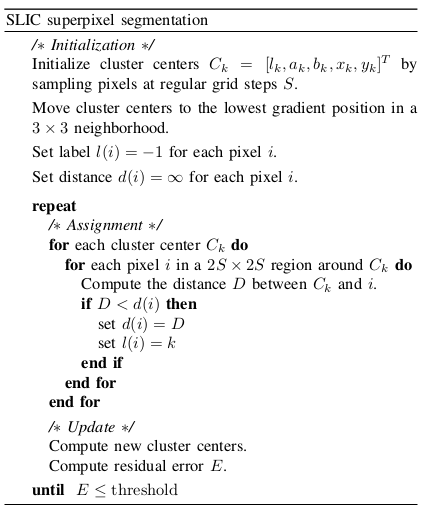
\includegraphics[width=.5\textwidth]{algoritmo_slic.png}
\caption{Algoritmo SLIC - Adaptado de \cite{SLIC}}
\label{alg:SLIC}
\end{figure}



\subsubsection{Complexidade}


\subsubsection{Medida de Distância} 

\subsubsection{Outras Características} 


\subsection{Segmentação} \label{ssec:segmentacao}

\subsection{Redes Neurais} \label{ssec:redes_neurais}


%%%%%%%%%%%%%%%%%%%%%%%%%%%%%%%%%%%%%%%%%%%%%%%%%%%%%%%
%%%%%%%%%%%%%%%%%%%%%%%%%%%%%%%%%%%%%%%%%%%%%%%%%%%%%%%
%%%%%%%%%%%%%%%%%%%%%%%%%%%%%%%%%%%%%%%%%%%%%%%%%%%%%%%

\section{Materiais e Métodos} \label{sec:mat_metodos}

%%%%%%%%%%%%%%%%%%%%%%%%%%%%%%%%%%%%%%%%%%%%%%%%%%%%%%%
%%%%%%%%%%%%%%%%%%%%%%%%%%%%%%%%%%%%%%%%%%%%%%%%%%%%%%%
%%%%%%%%%%%%%%%%%%%%%%%%%%%%%%%%%%%%%%%%%%%%%%%%%%%%%%%

\section{Testes, Resultados e Discussões} \label{sec:testes}

%%%%%%%%%%%%%%%%%%%%%%%%%%%%%%%%%%%%%%%%%%%%%%%%%%%%%%%
%%%%%%%%%%%%%%%%%%%%%%%%%%%%%%%%%%%%%%%%%%%%%%%%%%%%%%%

\subsection{Subsections}


\begin{table}[ht]
\centering
\caption{Variables to be considered on the evaluation of interaction
  techniques}
\label{tab:exTable1}
\smallskip
\begin{tabular}{|l|c|c|}
\hline
& Value 1 & Value 2\\[0.5ex]
\hline
&&\\[-2ex]
Case 1 & 1.0 $\pm$ 0.1 & 1.75$\times$10$^{-5}$ $\pm$ 5$\times$10$^{-7}$\\[0.5ex]
\hline
&&\\[-2ex]
Case 2 & 0.003(1) & 100.0\\[0.5ex]
\hline
\end{tabular}
\end{table}

%%%%%%%%%%%%%%%%%%%%%%%%%%%%%%%%%%%%%%%%%%%%%%%%%%%%%%%
%%%%%%%%%%%%%%%%%%%%%%%%%%%%%%%%%%%%%%%%%%%%%%%%%%%%%%%
%%%%%%%%%%%%%%%%%%%%%%%%%%%%%%%%%%%%%%%%%%%%%%%%%%%%%%%

\section{Conclusão} \label{sec:conclusao}

%%%%%%%%%%%%%%%%%%%%%%%%%%%%%%%%%%%%%%%%%%%%%%%%%%%%%%%
%%%%%%%%%%%%%%%%%%%%%%%%%%%%%%%%%%%%%%%%%%%%%%%%%%%%%%%
%%%%%%%%%%%%%%%%%%%%%%%%%%%%%%%%%%%%%%%%%%%%%%%%%%%%%%%

\bibliographystyle{sbc}
\bibliography{sbc-template}

\end{document}
